\subsubsection{UC7 - Visione ad alto livello - utente autenticato}
\begin{figure}[h]
	\centering
	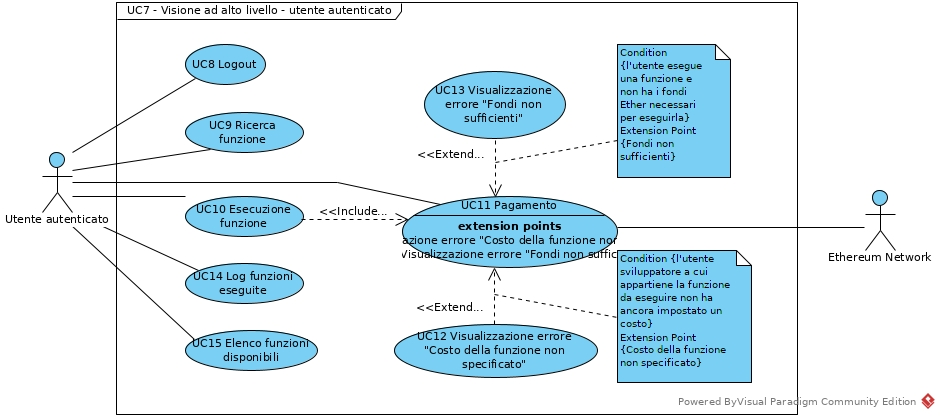
\includegraphics[width=\linewidth]{res/img/UC7.jpg}
	\caption{Diagramma visione ad alto livello - utente autenticato}
\end{figure}
\begin{itemize}
	\item \textbf{Attori primari:} Utente autenticato;
	\item \textbf{Attori secondari:} \textit{Ethereum\glo} network;
	\item \textbf{Descrizione:} l'utente che ha eseguito l'autenticazione a \textit{Etherless} mediante l'utenza \textit{Ethereum\glo} potrà eseguire i comandi relativi ad un utente utilizzatore;
	\item \textbf{Pre-condizioni:} l'utente ha eseguito l'accesso al sistema;
	\item \textbf{Post-condizioni:} l'utente potrà eseguire i comandi messi a disposizione per gli utenti utilizzatori della piattaforma;
	\item \textbf{Scenario principale:}
	\begin{enumerate}
		\item L'utente può eseguire il logout da \textit{Etherless} (UC8);
		\item L'utente può cercare i dettagli di una funzione presente nel sistema (UC9);
		\item L'utente può eseguire una funzione presente nel sistema (UC10);
		\item L'utente può pagare allo sviluppatore della funzione e ai gestori del servizio una somma in \textit{Ether\glo} per aver eseguito una determinata funzione (UC11);
		\item L'utente può visualizzare errori relativi al pagamento per "fondi non sufficienti" (UC13);
		\item L'utente può visualizzare errori relativi al pagamento per "costo della funzione non specificato" (UC12);
		\item L'utente può eseguire il log delle funzioni da lui eseguite (UC14);
		\item L'utente può visualizzare l'elenco delle funzioni disponibili nel sistema (UC15).
	\end{enumerate}
\end{itemize}
